\documentclass{article}
\usepackage{tikz}
\usetikzlibrary{external}
\tikzexternalize[mode=list and make]

\tikzset{
    % Defines a custom style which generates BOTH, .pdf and .png export
    % but prefers the .png on inclusion.
    %
    % This style is not pre-defined, you may need to copy-paste and
    % adjust it.
    png export/.style={
        external/system call/.add={}{; convert -density 300 -transparent white "\image.pdf" "\image.png"},
        %
        /pgf/images/external info,
        /pgf/images/include external/.code={%
            \includegraphics
            [width=\pgfexternalwidth,height=\pgfexternalheight]
            {##1.png}%
        },
    },
    %
    png export,% ACTIVATE
}

\begin{document}

{
% Here we specify the figure will be converted and inserted as PNG
\tikzset{png export}
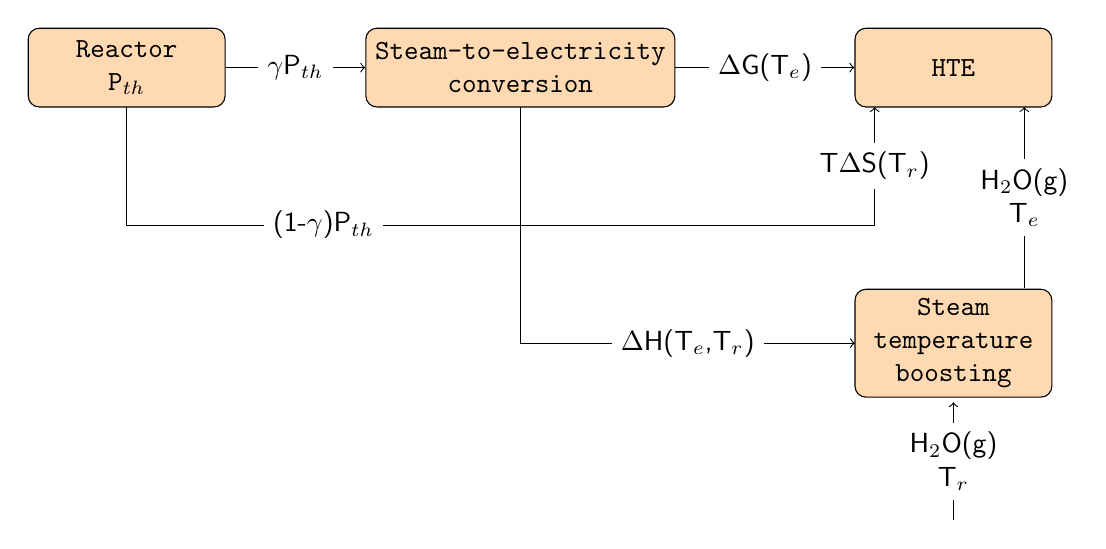
\begin{tikzpicture}[
    base/.style = {rectangle, rounded corners, draw=black,
minimum width=3cm, minimum height=1cm,
text centered, font=\sffamily},
process/.style = {base, minimum width=2.5cm, fill=orange!30,
font=\ttfamily},
node distance=3cm,
every node/.style={fill=white, font=\sffamily}, align=center
]

  \node (reactor) [process] {Reactor\\P$_{th}$};
  \node (steam1)  [process, right of=reactor, xshift=2.cm] {Steam-to-electricity\\conversion};
  \node (hte)     [process, right of=steam1, xshift=2.5cm] {HTE};
  \node (steam2)  [process, below of=hte, yshift=-0.5cm, xshift=0.cm] {Steam\\temperature\\boosting};
  
  \draw[->]     (reactor) -- (steam1) node[midway] {$\gamma$P$_{th}$};
  \draw[->]     (reactor) ++(0.,-0.5)-- ++(0.,-1.5)-- node[midway] {(1-$\gamma$)P$_{th}$} ++(5,0)-- ++(4.5,0.)-- node[midway] {T$\Delta$S(T$_r$)} ++(0.,1.5);
  \draw[->]     (steam1) ++(0,-.5)-- ++(0.,-3.)-- node[midway] {$\Delta$H(T$_e$,T$_r$)} ++(4.25,0.);
  \draw[->]     (steam1) -- (hte) node[midway] {$\Delta$G(T$_e$)};
  
  \draw[->]     (steam2) ++(0,-2.25)-- node[midway] {H$_2$O(g)\\T$_r$} ++(0,1.5);
  \draw[->]     (steam2) ++(0.9,0.7)-- node[midway] {H$_2$O(g)\\T$_e$} ++(0,2.3);

\end{tikzpicture}
}

{
% Here we specify the figure will be converted and inserted as PNG
\tikzset{png export}
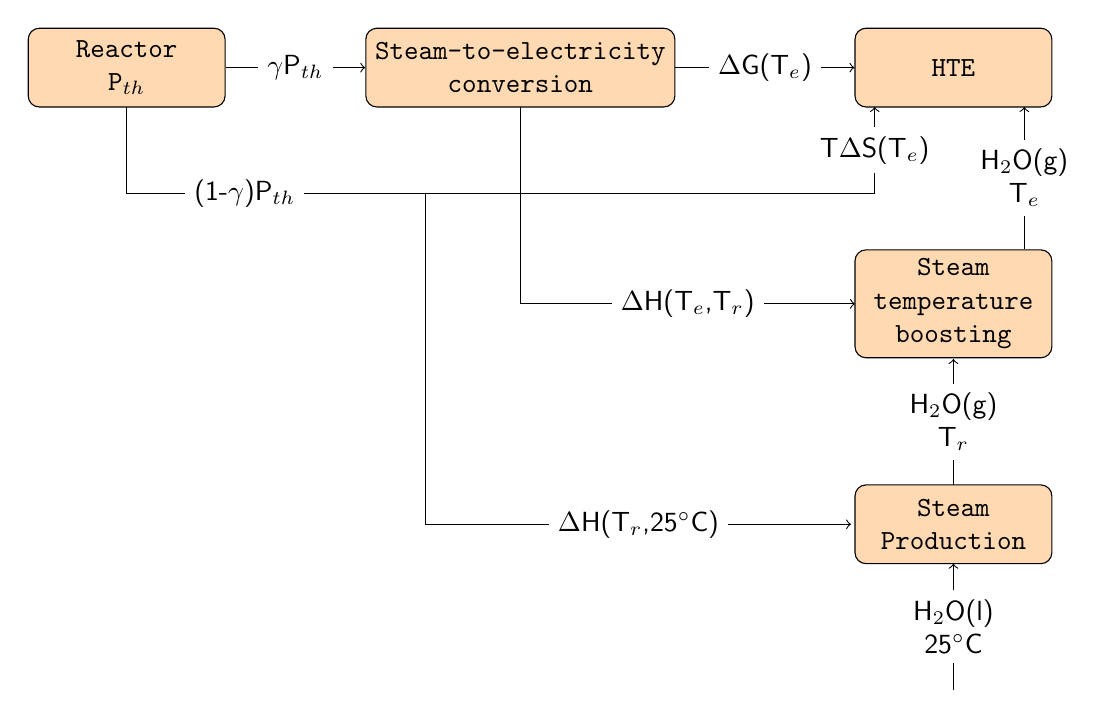
\begin{tikzpicture}[
    base/.style = {rectangle, rounded corners, draw=black,
minimum width=3cm, minimum height=1cm,
text centered, font=\sffamily},
process/.style = {base, minimum width=2.5cm, fill=orange!30,
font=\ttfamily},
node distance=3cm,
every node/.style={fill=white, font=\sffamily}, align=center
]

  \node (reactor) [process] {Reactor\\P$_{th}$};
  \node (steam1)  [process, right of=reactor, xshift=2.cm] {Steam-to-electricity\\conversion};
  \node (hte)     [process, right of=steam1, xshift=2.5cm] {HTE};
  \node (steam2)  [process, below of=hte, yshift=0cm, xshift=0.cm] {Steam\\temperature\\boosting};
  \node (steam3)  [process, below of=steam2, yshift=0.2cm, xshift=0.cm] {Steam\\Production};
  
  \draw[->]     (reactor) -- (steam1) node[midway] {$\gamma$P$_{th}$};
  \draw[->]     (reactor) ++(0.,-0.5)-- ++(0.,-1.1)-- node[midway] {(1-$\gamma$)P$_{th}$} ++(3,0)-- ++(6.5,0.)-- node[midway] {T$\Delta$S(T$_e$)} ++(0.,1.1);
  \draw[->]     (steam1) ++(0,-.5)-- ++(0.,-2.5)-- node[midway] {$\Delta$H(T$_e$,T$_r$)} ++(4.25,0.);
  \draw[->]     (steam1) -- (hte) node[midway] {$\Delta$G(T$_e$)};
  
  \draw[->]     (steam2) ++(0,-2.3)-- node[midway] {H$_2$O(g)\\T$_r$} ++(0,1.6);
  \draw[->]     (steam2) ++(0.9,0.7)-- node[midway] {H$_2$O(g)\\T$_e$} ++(0,1.8);

  \draw[->]     (reactor) ++(3.8,-1.6)-- ++(0,-4.2)-- node[midway] {$\Delta$H(T$_r$,25$^\circ$C)} ++(5.4,0);
  \draw[->]     (steam3) ++(0,-2.1)-- node[midway] {H$_2$O(l)\\25$^\circ$C} ++(0,1.6);

\end{tikzpicture}
}

\end{document}

% To compile do make; make -f hte1.makefile


